%%%%%%%%%%TO FORMAT A PREPRINT When accepted by a PCI%%%%%%%%%%%%%%%%
%%%%%%%%%%%%%%%%%%%%%%%%%%%%%%%%%%%%%%%%%%%%%%

\documentclass[a4paper]{article}

%%% [IF ACCEPTED] CHOOSE A PCI  %%%%%%%%%%%%%%%%%%%%%%%%%%%%%%%%%%%%%%%%%%%%%
%\newcommand{\PCI}{Peer Community In Zoology}
%\newcommand{\PCI}{Peer Community In Ecology}
%\newcommand{\PCI}{Peer Community In Evolutionary Biology}
%\newcommand{\PCI}{Peer Community In Paleontology}
%\newcommand{\PCI}{Peer Community In Archaeology}
%\newcommand{\PCI}{Peer Community In Animal Science}
%\newcommand{\PCI}{Peer Community In Genomics}
%\newcommand{\PCI}{Peer Community In Neuroscience}
%\newcommand{\PCI}{Peer Community In Mathematical and Computational Biology}
\newcommand{\PCI}{Peer Community In Forest and Wood Sciences}
%\newcommand{\PCI}{Peer Community In Ecotoxicology and Environmental Chemistry}
%\newcommand{\PCI}{Peer Community In Infections}
%\newcommand{\PCI}{Peer Community In Registered Reports}
%\newcommand{\PCI}{Peer Community In Network Science}
%\newcommand{\PCI}{Peer Community In Microbiology}


%%%%%%%%%%%%%%%%%%%%%%%%%%%%%%%%%%%%%%%%%%%%%%%%%%%%%%%%%%%%%%%%%%%%%%%%%%%%%

%%%%%%%%% [IF ACCEPTED] CHOOSE A BADGE [IF ACCEPTED]  %%%%%%%%%%%%%%%%%%%%%%%%%%%%%%%%%%%%%%%%%%%%%
%Comment lines 132 and/or 134 in preambule.tex if you don't use data and/or code in your preprint
%%%%%%%%%%%%%%%%%%%%%%%%%%%%%%%%%%%%%%%%%%%%%%%%%%%%%%%%%%%%%%%%%%%%%%%%%%%%%


%%%%%%%%%   SET THE TITLE   %%%%%%%%%%%%%%%%%%%%%%%%%%%%%%%%%%%%%%%%%%%%%
\newcommand{\preprinttitle}{This is the title of the preprint}
%%%%%%%%%%%%%%%%%%%%%%%%%%%%%%%%%%%%%%%%%%%%%%%%%%%%%%%%%%%%%%%%%%%%%%%%%%%%%

%%%%%%%%% [IF ACCEPTED] SET THE version of the preprint. Replace X by a number  [IF ACCEPTED] %%%%%%%%%%%%%%%%%%%%%%%%%%%%%%%%%%%%%%%%%%%%%
\newcommand{\version}{X}
%%%%%%%%%%%%%%%%%%%%%%%%%%%%%%%%%%%%%%%%%%%%%%%%%%%%%%%%%%%%%%%%%%%%%%%%%%%%%


%%%%%%%%%  SET THE LIST OF AUTHORS WITH CORRESPONDING AFFILIATIONS  use \& before last author %%%%%%%%%%%%%%%%%%%%
\newcommand{\listauthors}{\raggedright 
FirstnameOne FamilynameOne\textsuperscript{1}, \space
FirstnameTwo FamilynameTwo\textsuperscript{1}, \&
FirstnameThree FamilynameThree\textsuperscript{2}
%\fourthauthor \textsuperscript{i}
%etc...
}
%%%%%%%%%%%%%%%%%%%%%%%%%%%%%%%%%%%%%%%%%%%%%%%%%%%%%%%%%%%%%%%%%%%%%%%%%%%%%



%%%%%%%%%%%%%%%%%%%%%%%%%%%%%  SET THE LIST OF AFFILIATIONS  %%%%%%%%%%%%%%%%%%%%
\newcommand{\listinstitutions}{
\textsuperscript{1} DeptOne, InstitutionOne -- TownOne, CountryOne 
\\
\textsuperscript{2} DeptTwo, InstitutionTwo -- TownTwo, CoutryTwo
%\\
%\textsuperscript{3} \thirdinstitution
%etc
}
%%%%%%%%%%%%%%%%%%%%%%%%%%%%%%%%%%%%%%%%%%%%%%%%%%%%%%%%%%%%%%%%%%%%%%%%%%%%%


%%%%%%%%%%%%%%%%%%%%%%%%% [IF ACCEPTED] SET THE DATE OF UPLOAD on the preprint server  [IF ACCEPTED] %%%%%%%%%%%%%%
\newcommand{\datepub}{ddth Month yyyy}
%%%%%%%%%%%%%%%%%%%%%%%%%%%%%%%%%%%%%%%%%%%%%%%%%%%%%%%%%%%%%%%%%%%%%%%%%%%%%


%%%%%%%%%%%%%%%%%%%%%%%%% [IF ACCEPTED] SET THE RECOMMENDER(s) NAME(s) [IF ACCEPTED] %%%%%%%%%%%%%%
\newcommand{\recommender}{FirstName FamilyName}
%%%%%%%%%%%%%%%%%%%%%%%%%%%%%%%%%%%%%%%%%%%%%%%%%%%%%%%%%%%%%%%%%%%%%%%%%%%%%

%%%%%%%%%%%%%%%%%%%%%%%%% [IF ACCEPTED] SET THE DOI of the RECOMMENDATION  [IF ACCEPTED] %%%%%%%%%%%%%%
\newcommand{\DOIrecommendation}{xxx/xxx}
%%%%%%%%%%%%% for example 10.24072/pci.mcb.100003 %%%%%%%%%%%%%%%%%%%%%%%%



%%%%%%%%%%%%%%%%%%%%%%%%% [IF ACCEPTED] SET THE REVIEWERS' NAMES IF KNOWN and/or X anonymous reviewers  [IF ACCEPTED] %%%%%%%%%%%%%%
\newcommand{\reviewers}{FirstName FamilyName and two anonymous reviewer}
%%%%%%%%%%%%%%%%%%%%%%%%%%%%%%%%%%%%%%%%%%%%%%%%%%%%%%%%%%%%%%%%%%%%%%%%%%%%%



%%%%%%%%%%%%%%%%%%%%%   [IF ACCEPTED] SET THE 'CITE AS' OF YOUR PREPRINT. paste the line we sent you by Email (XXX the "cite as") in place of the xxx  [IF ACCEPTED] %%%%%%%%%%%%
\newcommand{\citeas}{xxx}
%%%%%%%%%%%%%%%%%%%%%%%%%%%%%%%%%%%%%%%%%%%%%%%%%%%%%%%%%%%%%%%%%%%%%%%%%%%%%


%%%%%%%%%%%%%%%%%%%%%%%%%%%%%%%%%  SET THE 'CORRESPONDENCE TO' %%%%%%%%%%%%%%%%%
\newcommand{\email}{mail.mail@mail.xx}
%%%%%%%%%%%%%%%%%%%%%%%%%%%%%%%%%%%%%%%%%%%%%%%%%%%%%%%%%%%%%%%%%%%%%%%%%%%%%

%%%%%%%%%%%%%%%%%%%%%%%%%%%%%%%%%  SET THE ABSTRACT %%%%%%%%%%%%%%%%%
\newcommand{\preprintabstract}{This is the abstract. This is the abstract. This is the abstract. This is the abstract. This is the abstract. This is the abstract. This is the abstract. This is the abstract. This is the abstract. This is the abstract. This is the abstract. This is the abstract. This is the abstract. This is the abstract. This is the abstract. This is the abstract. This is the abstract. This is the abstract. This is the abstract. This is the abstract. This is the abstract. This is the abstract. This is the abstract. This is the abstract. This is the abstract. This is the abstract. This is the abstract. This is the abstract. This is the abstract. This is the abstract. This is the abstract. This is the abstract. This is the abstract. This is the abstract. This is the abstract. This is the abstract. This is the abstract. This is the abstract. This is the abstract. This is the abstract. This is the abstract. This is the abstract. This is the abstract. This is the abstract.This is the abstract. This is the abstract. This is the abstract. This is the abstract. This is the abstract. This is the abstract. This is the abstract. This is the abstract. This is the abstract. This is the abstract. This is the abstract. This is the abstract. This is the abstract. This is the abstract. This is the abstract. This is the abstract. This is the abstract. This is the abstract. This is the abstract. This is the abstract. This is the abstract. This is the abstract.}
%%%%%%%%%%%%%%%%%%%%%%%%%%%%%%%%%%%%%%%%%%%%%%%%%%%%%%%%%%%%%%%%%%%%%%%%%%%%%

%%%%%%%%%%%%%%%%%%%%%%%%%%%%%%%%%  SET THE KEYWORDS %%%%%%%%%%%%%%%%%
\newcommand{\preprintkeywords}{KeywordOne; KeywordTwo; KeywordThree; KeywordFour; KeywordFive}
%%%%%%%%%%%%%%%%%%%%%%%%%%%%%%%%%%%%%%%%%%%%%%%%%%%%%%%%%%%%%%%%%%%%%%%%%%%%%

%%%%%%%%%%TO FORMAT A PREPRINT%%%%%%%%%%%%%%%%
%%%%%%%%%%%%%%%%%%%%%%%%%%%%%%%%%%%%%%%%%%%%%%
%%%%%%%%%%%%%%%%%%%%%%%%%%%%%%%%%%%%%%%%%%%%%%

\usepackage[margin=1in,marginparwidth=4.2cm,marginparsep=0.5cm]{geometry}

\usepackage{marginnote}
\usepackage{pdflscape}
\usepackage{ifthen}
\reversemarginpar  % sets margin notes to the left
\usepackage{lipsum} % Required to insert dummy text
\usepackage{calc}
\usepackage{siunitx}
\usepackage[right]{lineno}
\usepackage{titlesec}
\usepackage{indentfirst}
%\usepackage[none]{hyphenat} % use only if there is a problem
% Use Unicode characters
\usepackage[utf8]{inputenc}
\usepackage[T1]{fontenc}
% Clean citations with biblatex
\usepackage[
backend=biber,
natbib=true,
sortcites=true,
defernumbers=true,
style=authoryear,
citestyle=authoryear-comp,
maxnames=99,
maxcitenames=2,
uniquename=init,
giveninits=true,
terseinits=true,
url=false
]{biblatex}
\DeclareNameAlias{default}{family-given}
\renewcommand*{\revsdnamepunct}{} % no comma between family and given names
\renewbibmacro{in:}{%
  \ifentrytype{article}{}{\printtext{\bibstring{in}\intitlepunct}}} % remove 'In:' before journal name
\DeclareFieldFormat[article]{pages}{#1} % remove pp.
\AtEveryBibitem{\ifentrytype{article}{\clearfield{number}}{}} % don't print issue numbers
\DeclareFieldFormat[article, inbook, incollection, inproceedings, misc, thesis, unpublished]{title}{#1} % title without quotes
\usepackage{csquotes}
\RequirePackage[english]{babel} % must be called after biblatex
\addbibresource{sample.bib}
\DeclareBibliographyCategory{ignore}
\addtocategory{ignore}{recommendation} % adding recommendation to 'ignore' category so that it does not appear in the References
% Clickable references. Use \url{www.example.com} or \href{www.example.com}{description} to add a clicky url
\usepackage{nameref}
\usepackage[pdfborder={0 0 0}]{hyperref}  % sets link border to white
\urlstyle{same}



% Include figures
\usepackage{graphbox}  % loads graphicx ppackage with extended options for vertical alignment of figures
% Improve typesetting in LaTex
\usepackage{microtype}
\DisableLigatures[f]{encoding = *, family = * }
% Text layout and font (Open Sans)
\setlength{\parindent}{0.4cm}
\linespread{1.2}
\RequirePackage[default,scale=0.90]{opensans}
% Defining document colors
\usepackage{xcolor}
\definecolor{darkgray}{HTML}{808080}
\definecolor{mediumgray}{HTML}{6D6E70}
\definecolor{ligthgray}{HTML}{d9d9d9}
\definecolor{pciblue}{HTML}{74adca}
\definecolor{opengreen}{HTML}{77933c}
% Use adjustwidth environment to exceed text width
\usepackage{changepage}
% Adjust caption style
\usepackage[aboveskip=1pt,labelfont=bf,labelsep=period,singlelinecheck=off]{caption}

% Headers and footers


% DOI's
\newcommand{\DOIlink}{\href{https://doi.org/\DOI}{https://doi.org/\DOI}}
\newcommand{\DOIrecommendationlink}{\href{https://doi.org/\DOIrecommendation}{https://doi.org/\DOIrecommendation}}

\newcommand{\beginingpreprint}{
\vspace*{0.5cm}
\begin{flushleft}
\baselineskip=0pt

{\Huge
\fontseries{sb}\selectfont{\preprinttitle}}
\end{flushleft}
\vspace*{0.25cm}
\begin{flushleft}
\Large
\listauthors
\end{flushleft}
\bigskip
{\raggedright
\listinstitutions}
\\
\\
\textbf{Correspondence: } \href{mailto:\email}{\email}\\
\\
\vspace*{0.5cm}
\fcolorbox{pciblue}{pciblue}{
\parbox{\textwidth - 2\fboxsep}{
\vspace{0.25cm}
\begin{internallinenumbers}
\textbf{\large{\textsc{Abstract}}}\\

\preprintabstract\\

\textbf{\emph{Keywords: }}\preprintkeywords
\end{internallinenumbers}

\vspace{0.25cm}}
}
\newpage
\newgeometry{margin=1in}
}






\begin{document}
\beginingpreprint

%%%%%%%%%%%%%%%%%%%%%  [IF ACCEPTED] comment linenumbers %%%%%%%%%%%%%
%\linenumbers

%%%%% Text of the preprint %%%%%%
% use \emph{} for italics and \parencite{} to cite a reference and \ref{XX} to cite the \label{XX}
% use \\ and a blank line to mark the end of paragraph and starting of a new one

\section*{\centering Introduction}

This is an example of text. This realization is especially important because it can flip around our expectations about which species expand fast, and how to manage them. We tend to think of initial colonization and long-term abundance as two independent axes of variation among species or indeed as two ends of a spectrum, in the classic competition-colonization tradeoff \parencite{levins1971regional}. When both play into invasion speed, good dispersers might not outrun good competitors. This is useful knowledge, whether we want to contain an invasion or secure a reintroduction. \\ 

In their study "When higher carrying capacities lead to faster propagation", \textcite{levins1971regional} combine mathematical analysis, Individual-Based simulations and experiments to show that various mechanisms can cause pushed fronts, whose speed increases with the carrying capacity K of the species. Rather than focus on one particular angle, the authors endeavor to demonstrate that this qualitative effect appears again and again in a variety of settings. \\

It is perhaps surprising that this notable and general connection between K and invasion speed has managed to garner so little fame in ecology. A large fraction of the literature employs the venerable Fisher-KPP reaction-diffusion model, which combines local logistic growth with linear diffusion in space. This model has prompted both considerable mathematical developments \parencite{crooks2004spatial} and many applications to modelling real invasions \parencite{shigesada1997biological}. But it only allows pulled fronts, driven by the small populations at the edge of a species range, with a speed that depends only on their initial growth rate r.\\

\section*{\centering Material and methods}

This classic setup is, however, singular in many ways. \textcite{levins1971regional} use it as a null model, and introduce three mechanisms or factors that each ensure a 1 role of K in invasion speed, while giving less importance to the pioneers at the border. \\ 

Two factors, the Allee effect and demographic stochasticity, make small edge populations slower to grow or less likely to survive. These two factors are studied theoretically, and to make their claims stronger, the authors stack the deck against K. When generalizing equations or simulations beyond the null case, it is easy to obtain functional forms where the parameter K does not only play the role of equilibrium carrying capacity, but also affects dynamical properties such as the maximum or mean growth rate. In that case, it can trivially change the propagation speed, without it meaning anything about the role of established populations behind the front. \textcite{levins1971regional} avoid this pitfall by disentangling these effects, at the cost of slightly more peculiar expressions, and show that varying essentially nothing but the carrying capacity can still impact the speed of the invasion front. \\ 

\section*{\centering Results}
The third factor, density-dependent dispersal, makes small populations less prone to disperse. It is well established empirically (see Fig~\ref{Fig1}) and theoretically that various biological mechanisms, from collective organization to behavioral switches, can prompt organisms in denser populations to disperse more, e.g. in such a way as to escape competition \parencite{matthysen2005density}. The authors demonstrate how this effect induces a link between carrying capacity and invasion speed, both theoretically and in a dispersal experiment on the parasitoid wasp, \emph{Trichogramma chilonis}.\\ 


%%%%%% EXAMPLE OF A FIGURE   %%%%%%
\begin{figure}[h]
  \captionsetup{justification=centering}
  \caption{A nice picture of bidule.}
  \centering
  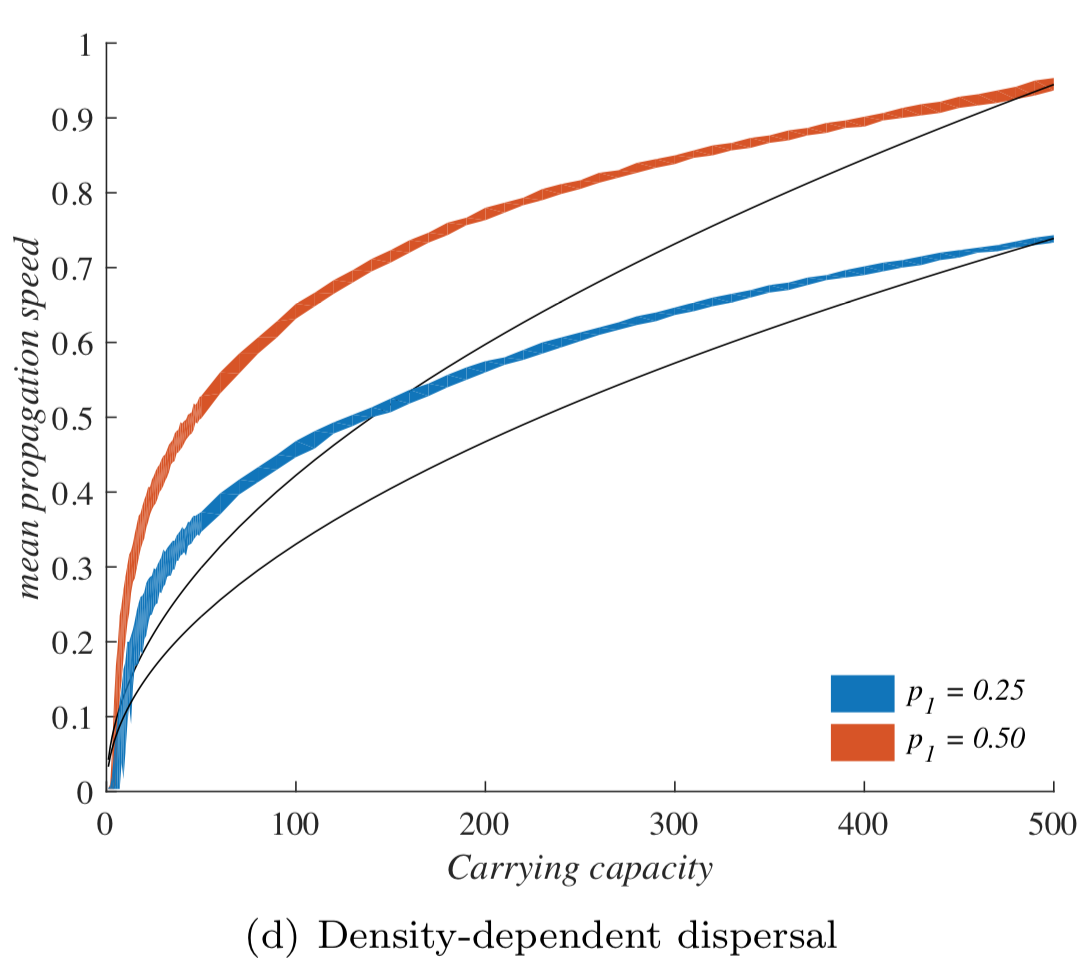
\includegraphics[scale=0.5]{fig.png}
  \label{Fig1}
\end{figure}
%%%%%%%%%%%%%%%%%%%%%%%%%%%%%%%%%%%

The third factor, density-dependent dispersal, makes small populations less prone to disperse. It is well established empirically (see Fig~\ref{Fig1}) and theoretically that various biological mechanisms, from collective organization to behavioral switches, can prompt organisms in denser populations to disperse more, e.g. in such a way as to escape competition \parencite{matthysen2005density}. The authors demonstrate how this effect induces a link between carrying capacity and invasion speed, both theoretically and in a dispersal experiment on the parasitoid wasp, \emph{Trichogramma chilonis}.\\ 
The third factor, density-dependent dispersal, makes small populations less prone to disperse. It is well established empirically (see Fig~\ref{Fig1}) and theoretically that various biological mechanisms, from collective organization to behavioral switches, can prompt organisms in denser populations to disperse more, e.g. in such a way as to escape competition \parencite{matthysen2005density}. The authors demonstrate how this effect induces a link between carrying capacity and invasion speed, both theoretically and in a dispersal experiment on the parasitoid wasp, \emph{Trichogramma chilonis}.\\ 
The third factor, density-dependent dispersal, makes small populations less prone to disperse. It is well established empirically (see Fig~\ref{Fig1}) and theoretically that various biological mechanisms, from collective organization to behavioral switches, can prompt organisms in denser populations to disperse more, e.g. in such a way as to escape competition \parencite{matthysen2005density}. The authors demonstrate how this effect induces a link between carrying capacity and invasion speed, both theoretically and in a dispersal experiment on the parasitoid wasp, \emph{Trichogramma chilonis}.\\ 

%%%%%%%%%% example of a page in landscape %%%%%%%%%%%%%
\begin{landscape}

This is a landscape page. The third factor, density-dependent dispersal, makes small populations less prone to disperse. It is well established empirically (see Fig~\ref{Fig1}) and theoretically that various biological mechanisms, from collective organization to behavioral switches, can prompt organisms in denser populations to disperse more, e.g. in such a way as to escape competition \parencite{matthysen2005density}. The authors demonstrate how this effect induces a link between carrying capacity and invasion speed, both theoretically and in a dispersal experiment on the parasitoid wasp, \emph{Trichogramma chilonis}.\\
The third factor, density-dependent dispersal, makes small populations less prone to disperse. It is well established empirically (see Fig~\ref{Fig1}) and theoretically that various biological mechanisms, from collective organization to behavioral switches, can prompt organisms in denser populations to disperse more, e.g. in such a way as to escape competition \parencite{matthysen2005density}. The authors demonstrate how this effect induces a link between carrying capacity and invasion speed, both theoretically and in a dispersal experiment on the parasitoid wasp, \emph{Trichogramma chilonis}.\\

\end{landscape}
%%%%%%%%%%%%%%%%%%%%%%%%%%%%%%%%%%%%%%%%%%%%%%%%%%%%%

\section*{\centering Discussion}
Overall, this study carries a simple and clear message, supported by valuable contributions from different angles. Although some sections are clearly written for the theoretical ecology crowd, this article has something for everyone, from the stray physicist to the open-minded manager. The collaboration between theoreticians and experimentalists, while not central, is worthy of note. Because the narrative of this study is the variety of mechanisms that can lead to the same qualitative effect, the inclusion of various approaches is not a gimmick, but helps drive home its main message. The work is fairly self-contained, although one could always wish for further developments, especially in the direction of more quantitative testing of these mechanisms. \\ 

In conclusion, \textcite{levins1971regional} effectively convey the widely relevant message that, for some species, invading is not just about the destination, it is about the many offspring one makes along the way. \\ 


\section*{\centering Acknowledgements}
This is your acknowledgments.

\section*{\centering Fundings}
Your fundings.


\section*{\centering Conflict of interest disclosure}
The authors of this article declare that they have no financial conflict of interest with the content of this article. XXX and XXX are recommenders for PCI XXX

\section*{\centering Data, script and code availability}
Data are available online: DOI of the webpage hosting the data (or link)

\section*{\centering Supplementary information availability}
Script and codes are available online: DOI of the webpage hosting the script and codes (or link)


\section*{\centering Annexes or Supplementary Information}
This is your annex 1 if any

This is your annex 2 if any

\titleformat*{\section}{\bfseries\Large\centering}

%%%%%% if they exist, DOIs are required %%%%%%%
\printbibliography[notcategory=ignore]

\end{document}
